\documentclass[a4paper,10pt]{scrartcl}
\usepackage[utf8]{inputenc}
\usepackage{booktabs}
\usepackage{tabularx}
\usepackage{graphicx}
\usepackage{listings}
\usepackage[table]{xcolor}
\usepackage{amsmath}
\usepackage{multicol}
\usepackage{todonotes}
\usepackage{geometry}
\usepackage{cleveref}
\usepackage{longfbox}
\usepackage{enumitem}
% \usepackage[table,xcdraw]{xcolor}
% \usepackage[most]{tcolorbox}

\definecolor{listinggray}{gray}{0.9}
\definecolor{lbcolor}{rgb}{0.9,0.9,0.9}
\definecolor{llbcolor}{rgb}{0.97,0.97,0.97}

\lstdefinelanguage{GTClang}{
language     = C++,
keywordstyle = [1]{\color[RGB]{140,45,4}},
keywordstyle = [2]{\color[RGB]{254,153,41}},
keywordstyle = [3]{\color[RGB]{236,112,20}},
keywordstyle = [4]{\color[RGB]{204,76,2}},
keywordstyle = [5]{\color[RGB]{240,59,32}},
basicstyle=\footnotesize,
%  identifierstyle=\color{magenta},
stringstyle=\color{red}
commentstyle=\color{ForestGreen},
morekeywords = [1]{field},
morekeywords = [1]{offset},
morekeywords = [1]{temporary},
morekeywords = [2]{function},
morekeywords = [2]{computation},
morekeywords = [2]{globalVariable},
morekeywords = [3]{iterationSpace},
morekeywords = [3]{level},
morekeywords = [3]{topLevel},
morekeywords = [3]{bottomLevel},
morekeywords = [4]{neighbour_loop},
morekeywords = [4]{reduction},
morekeywords = [4]{neighbours},
morekeywords = [5]{edges},
morekeywords = [5]{center},
}
\lstset{
backgroundcolor=\color{llbcolor},
tabsize=4,
language=GTClang,
captionpos=b,
tabsize=3,
frame=lines,
numbers=left,
numberstyle=\tiny,
numbersep=5pt,
breaklines=true,
showstringspaces=false,
escapeinside={<@}{@>}
}

\definecolor{accesspattern}{RGB}{240,59,32}
\setlength\parindent{0pt}

\title{Preparation for the ESCAPE-2 Workshop on DSL concepts}
\author{Tobias Wicky, Oliver Fuhrer, Reinhard Budich, Carlos Osuna}

\geometry{left=3cm, right=2cm, bottom=30mm}
\begin{document}
\maketitle

%%%%%%%%%%%%%%%%%%%%%%%%%%%%%%%%%%%%%%%%%%%%%%%%%%%%%%%%55
\section{Workshop Checklist}

\begin{itemize}
	\item Bring the most common computational pattern ready to be presented and discussed in pseudo-code, Fortran, or any other language, but simple enough so that we can reason about it. Extract the relevant computational patterns by removing boiler-plate and unnecessary code.
	\item Focus on the most commonly used patterns, but dont forget to also consider corner cases, or more rare cases. Even if we focus on the most frequently used patterns, it is important to understand how much of the total application we are covering with these patterns. In the world of DSLs, exceptions to the rule are important!
	\item On the first day we will organize working groups where developers from models/methods with similar computational patterns would gather to discuss them and the compile a list of concepts that are required. Be ready to present your pseudo-code or reasoning to others in such a way that they can understand the essence of it.
	\item Reasoning about patterns and concepts is enough. We dont need functional, compiling and running applications.
	\item Feel free to invent your own personal high-level DSL and prepare you examples / algorithmic motifs directly in this DSLs.
\end{itemize}

%%%%%%%%%%%%%%%%%%%%%%%%%%%%%%%%%%%%%%%%%%%%%%%%%%%%%%%%55
\section{Introduction}

A domain-specific language for weather and climate applications must be built on top
of a set of concepts / language elements
that cover the employed algorithmic motifs of weather and climate codes.
A concise defintion of these concepts (in the form of a high-level intermediate representation)
will allow us to standardize and share programming tools, domain specific languages (DSLs),
source-to-source translators, etc. that allow to write
models in an expressive manner and generate efficient implementations
for multiple architectures.

With the involvement of key developers of different weather and climate
models, the goal of the workshop is to identify and define the required concepts
that will be needed to capture most of the computational
patterns present in weather and climate applications. The derived set of concepts will be used
to develop a high-level intermediate representation (HIR).

In this document we illustrate the process of identifying and deriving concepts 
for some particular computational patterns, to 
serve as a demonstration of how to infer the relevant concepts
to capture the important algorithmic motifs of the different numerical methods,
discretization schemes and grids that we plan to support.
It is not the goal to propose a particular solution. On the contrary the document
derives often multiple variants to motivate the discussion among the different developers.

\subsection{Characteristics of a good definition of concepts}

The following characteristics will be considered axioms of a good definition of concepts.
\label{sec:HIRDef}
\begin{enumerate}[label=\textbf{A.\arabic*}]
    \item Language independent 
    \item Complete, in the sense of supporting all the relevant applications of weather and climate that the community would like to support
    \item Hardware agnostic, no assumptions should be made on the hardware where it will run, like choosing a specific parallel model implementation. \label{A:hardware}
    \item Extensible / enrichable
    \item Simple
    \item Orthogonal, i.e. no redundancy of concepts \label{A:ortho}
\end{enumerate}

%%%%%%%%%%%%%%%%%%%%%%%%%%%%%%%%%%%%%%%%%%%%%%%%%%%%%%%%55
\section{Computational patterns}
\label{sec:comppatterns}

Following the characteristics given in \cref{sec:HIRDef}, this section will explain 
what are the relevant computational patterns and how to capture them into concepts of an HIR.

The idea is to extract a minimal set of orthogonal (\ref{A:ortho}) concepts with which we can express (unambiguously) the employed numerical methods on the underlying grid.

An specific efficient parallel implementation and the decisions taken (e.g., whether two loops are fused or not)
depends on the target computing architecture. Therefore the HIR should only cover high level concepts of a
descriptive language (DSL) that captures the computational patterns of the discretization, without attempting
to describe a parallel implementation (\ref{A:hardware}).
Details like where data storage order, organization of the loops, data dependency resolution can
either be carried out by the DSL toolchain.

A natural concept of HIR will be the statement, that would be equivalent to the update equation of a field. For example:
\begin{lstlisting}
forall i,j,k in domain:
  lap[i,j,k] = u[i+1,j,k] + u[i-1,j,k] + u[i,j+1,k] + u[i,j-1,k] - 4.0 * u[i,j,k]
\end{lstlisting}

\begin{longfbox}[rounded]
We can assume that our program will be a sequence of statements, executed in the order described (unless data
dependencies allow a reordering) which would produce a valid result if they would be executed sequentially.
%\footnote{Notice this approach follows the imperative programming paradigm, similar to the way the statements of today's weather models form a Fortran program. Other approaches like a pure function approach could be adopted. The discussion
%of the implications lies out of the scope of this document.}
\end{longfbox}

\subsection{Identify Characteristics of Computational Patterns}
\label{sec:idPattern}

\textbf{Data Structures:}\newline
All weather and climate models are computing on data that is multi-dimensional. Although there are considerable differences
from different methods/grids. Some questions that motivate the understanding of the data structure patterns follow:
\begin{itemize}
	\item What is the dimensionality of the data structures? How many dimensions are employed to represent prognostic variables or fields in the grid?
	\item Does each grid point store a builtin type, e.g. double, int, etc... or complex types?
	\item Is the dimensionality fixed or can it vary in different part of the code, or over time or in different areas of the grid (like in a mesh refinement approach)? 
	  \item Which dimensions are parallel (computations are independent along dimension) and which dimensions contain data dependencies by applying sequential solvers (e.g. Thomas algorithm for a tridiagonal solve)?
\end{itemize}

\textbf{Access Patterns:}\newline
Any computation will operate on a set input fields and write into an output field. This may for example be in a quasi-homogeneous manner through the whole grid, where input fields are only accesses in a compact neighbourhood of the grid location
of the output field being computed (e.g. stencil computations).

The questions related to the access patterns are:
\begin{itemize} 
  \item Are neighbouring grid points accessed? If no, your access pattern is very simple, otherwise the following
  questions will apply.
  \item Does the application access neighbours in all dimensions? 
  \item Do the computations access one level or neighbours or go beyond? Is it limited to certain extent, or can
  the application access any far away neighbour (e.g. semi-lagrangian methods, implicit methods)? Along which dimensions?
  \item Are accesses uniform through all the neighbours of a grid-point in the topology of the grid,
        like a sum over all adjoining grid cells,
	or on the contrary are there specific neighbour accesses, like an one-dimensional advection scheme (accessing only neighbours in a single dimension)?
  \item Are there absolute or relative indices?
  \item Is indirect indexing required?
\end{itemize}

\textbf{Computation:}\newline
\begin{itemize}
  \item Are the computations homogeneous in the whole grid, or are there specializations required for certain regions (e.g. boundary conditions, hybrid vertical coordinate systems, corners of a cubed sphere grid)? If so, where and in which dimensions?
  \item What kind of computational patterns are required? Some examples are: compact horizontal or 3D stencils, iterative solvers in one or more than one direction (e.g. Thomas algorithm), iterative solvers (e.g. conjugent gradient), reduction operations (e.g. computation of a residual)?
\end{itemize}

%%%%%%%%%%%%%%%%%%%%%%%%%%%%%%%%%%%%%%%%%%%%%%%%%%%%%%%%55
\section{Examples}

In this section we will analyze some examples of different computational patterns. From pseudo-code we will derive their properties and finally extract some concepts of an HIR that would be complete to describe the examples.
 
Pseudocode is used to emphasize that the specific definition of the language is not relevant.
Irrespective of whether the model is currently written in plain Fortran, an embedded DSL or a high-level DSL, the key concepts are the same.
In the pseudo-code, loops are not present. Following the assumptions made in \cref{sec:comppatterns} the statements of the pseudo-code are supposed to produced valid code when execute sequentially, and the equations update all the grid-points until covering the whole iteration space of the grid. 

\subsection{Example on a structured lat-lon grid}

The following example introduces computational patterns like those found in finite differences, finite volumes of a lat-lon grid. The grid is a cartesian 3-dimensional grid, with dimensions identified as $i,j,k$.

The following pseudo-code represents the computation of a filter or diffusion operator applied to a field

\begin{lstlisting}[label=lst:diff, caption=pseudo-code for a diffusion operator example]
computation diffusion {
  field u; 
  tmp lap;

  forall i,j,k in domain:
    lap[i,j,k] = u[i+1,j,k] + u[i-1,j,k] + u[i,j+1,k] + u[i,j-1,k] - 4.0 * u[i,j,k] <@\label{ln:lap}@>
  forall i,j,k in domain:
    u[i,j,k] = lap[i+1,j,k] + lap[i-1,j,k] + lap[i,j+1,k] + lap[i,j-1,k] - 4.0 * lap[i,j,k]
}
\end{lstlisting}

The following tables summarizes the analysis to the questions in \cref{sec:idPattern}:

\textbf{Data Structures:}\newline
\begin{itemize}
	\item What is the dimensionality of the data structures? How many dimensions are employed to represent prognostic variables or fields in the grid?
	
	\textcolor{orange}{$\rightarrow$ 3 dimensions in a cartesian grid (i,j,k)}
	
	\item Does each grid point store a builtin type, e.g. double, int, etc... or complex types?
	
	\textcolor{orange}{$\rightarrow$ builtin type, i.e. double, int...}
	
	\item Is the dimensionality fixed or can it vary in different part of the code, or over time or in different areas of the grid (like in a mesh refinement approach)?
	
	\textcolor{orange}{$\rightarrow$ fixed}
	
	\item Which dimensions are parallel (computations are independent along dimension) and which dimensions contain data dependencies by applying sequential solvers (e.g. Thomas algorithm for a tridiagonal solve)?
	
	\textcolor{orange}{$\rightarrow$ this operator can be parallelized in any of the 3 dimensions. However the application is domain decomposed in IJ only since in the rest of the application there are other tridiagonal solvers (using Thomas algorithm) in the K dimension (not visible from pseudo-code).} 
	
\end{itemize}

\textbf{Access Patterns:}\newline
\begin{itemize} 
	\item Are neighbouring grid points accessed?
	
	\textcolor{orange}{$\rightarrow$ yes}
	
	\item Does the application access neighbours in all dimensions? 
	
	\textcolor{orange}{$\rightarrow$ in general yes, although for this operator example only for IJ}
	
	\item Do the computations access one level or neighbours or go beyond? Is it limited to certain extent, or can the application access any far away neighbour (e.g. semi-lagrangian methods, implicit methods)? Along which dimensions?
	
	\textcolor{orange}{$\rightarrow$ in this operator, we access only one level of neighbours. In general, the application can access more than one, but nevertheless limited to a (configurable) maximum number of neighbours. Some computational
	patterns in the application access the full vertical column (K).}
	
	\item Are accesses uniform through all the neighbours of a grid-point in the topology of the grid, like a sum over all neighbour
	triangles, or on the contrary are there specific neighbour accesses, like an advection scheme on X dimension (accessing  only neighbours in the I dimension)?
	
	\textcolor{orange}{$\rightarrow$ this example is completely symmetric, however in the application there can be asymmetric operators, like one-dimensional advection in a single direction.}
	
	\item Are there absolute or relative indices?
	
	\textcolor{orange}{$\rightarrow$ all accesses are relative}
	
	\item Is indirect indexing required?
	
	\textcolor{orange}{$\rightarrow$ no}
\end{itemize}

\textbf{Computation:}\newline
\begin{itemize}
	\item Are the computations homogeneous in the whole grid, or are there specializations required for certain regions?
	If so, where and in which dimensions?
	
	\textcolor{orange}{$\rightarrow$ this example is applied uniformly to the whole grid. However a there are other
	examples in the application, like the following vertical average, that require specialization on the vertical dimension}
	
	\begin{lstlisting}
computation diffusion {
  field u, avg
  
  forall i,j in domain, for k = bottomLevel...topLevel-1:
    avg[i,j,k] = 0.5 * ( u[i,j,k+1] + u[i,j,k] )
  forall i,j in domain, for k = topLevel:
    avg[i,j,k] = u[i,j,k]
}
	\end{lstlisting}
	
	\item What kind of computational patterns are required? 
\end{itemize}

Given this analysis, the following set of concepts would be enough to provide a full specification of the example: 

\begin{enumerate}[label=\textbf{C.\arabic*}]
  \item \textbf{Dimensions}: this concept is needed to describe the existing dimensions (i,j,k).
  \item \textbf{Field declaration}: declares input/output fields of the computation as well as temporaries.
  \item \textbf{Field access with relative offsets in a cartesian grid}: allows to represent neighbour accesses like $u[i+1,j,k]$. \label{C:FieldAccess}
  \item \textbf{Iteration space}: parallel or sequential in arbitrary dimensions, allows to specialize the equations for different vertical regions.
\end{enumerate}

Like that, the computation of $lap$ in \cref{ln:lap} of \cref{lst:diff} can be expressed as \textit{sum of different field access with relative offsets}.

Alternatively, the same example could be presented in matrix formulation

\begin{lstlisting}
computation diffusion{
  field u
  temporary lap
  
  iterationSpace(i,j,k=topLevel,bottomLevel) {
<@\colorbox{lbcolor}{\hspace{0.6cm}lap = u$\begin{bmatrix}0 & 1 & 0\\1 & -4 & 1 \\0 & 1 & 0\end{bmatrix}$\hspace*{11.9cm}} @>
<@\colorbox{lbcolor}{\hspace{0.6cm}u = lap$\begin{bmatrix}0 & 1 & 0\\1 & -4 & 1 \\0 & 1 & 0\end{bmatrix}$\hspace*{11.7cm}} @>
  }
}
\end{lstlisting}

in which case, the \textit{sum of different field access with relative offsets} could be replaced by a new concept
\begin{itemize}
	\item \textbf{Stencil field access with a matrix of coefficients}, like $u\begin{bmatrix}0 & 1 & 0\\1 & -4 & 1 \\0 & 1 & 0\end{bmatrix}$
\end{itemize}

%%%%%%%%%%%%%%%%%%%%%%%%%%%%%%%%%%%%%%%%%%%%%%%%%%%%%%%%55
\subsection{Example for an unstructured mesh}

In this example, we present similar operators but implemented for an unstructured mesh, where the number of neighbours
are not fixed and can vary from grid point to grid point.

%%% TODO OLI: You say neighbors, but the figure shows a computation at the cell center and accesses edges, and not neighbors...

The example is shown in pseudo-code in \cref{lst:on_edges} and depicted in \cref{fig:on_edges}

\begin{lstlisting}[label=lst:on_edges, caption=Pseudo-code example of operator on neighbour grid points on an irregular grid]
computation div{
  field f, edge_length, div
  
  iterationSpace {
    div = reduction<neighbours>(f*edge_length, +)
  }
}
\end{lstlisting}

\begin{figure}[htp!]
	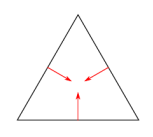
\includegraphics[width=4cm]{./on_edges.png}
	\caption{Example operator of a reduction on neighbour grid point elements}
	\label{fig:on_edges}
\end{figure}

The particularities of this example are:
\begin{enumerate}
	\item Accesses to neighbours are uniform. It does not customize weights for different neighbours
	\item The number of neighbours is not specified, the same operator could work on triangles, quadrilaterals, etc
	\item Dimensionality depends on the underlying grid. This operator applied to a structured lat-lon grid could
	be used with the same IJK dimensions. However when used for an (horizontal) unstructured mesh, only one dimension
	can be used for the horizontal, since there is no notion of row and columns.
\end{enumerate}

In this case, the concept of field access with relative offset (\cref{C:FieldAccess}) can
not be used to describe the neighbour operations. Instead we will need a new concept

\begin{enumerate}[label=\textbf{C.\arabic*}]
	  \setcounter{enumi}{4}
	\item \textbf{Reduction Over Neighbours}: this concept describes a reduction operation over neighbours,
	that contains an operator for reduction (sum in the example) and the field/fields on which it operates.
\end{enumerate}

Additionally, in the case of non-colocated grids, like shown also in \cref{fig:on_edges} we will need a concept
of location or function space (edges, vertices, faces,...), 
that describes where the fields are located. The reduction operation over neighbours will then be different
depending on the location of the output field and the location of the neighbour accesses.  
We will leave the exercise of extending the concepts to support non-colocated grids and 
possibly more complex operators over neighbours to the reader and developers of models that
contain these computational patterns. 

\end{document}
